% !TEX spellckeck=en_GB


\section{Introduction to autoencoders}\label{sec:intro_autoenc}

The primary challenge we face with data from the active target time projection chamber (AT-TPC) is that labelling data is not always possible for a given experiment. Given that fact, and the considerable amount of data available, we turn to dimensionality reduction methods to possibly express the different physics occurring in this data. One such set of methods is the autoencoder family of neural network algorithms.

An autoencoder is an attempt at learning a distribution of data by reconstruction. This goal means that the model encodes the data into a much lower dimensional latent space before projecting back into the original space of data. The goal, as a matter of course, is then to learn the true distribution, $P(\mathcal{X})$, over the data with some parametrized model $Q(\mathcal{X};\theta)$. The model consists of two discrete parts: an encoder and a decoder. The encoder is, in general, a nonlinear map $\psi$

\begin{align}
  \psi: \mathcal{X} \rightarrow \mathcal{Z},
\end{align}

\noindent where $\mathcal{X} $ and $\mathcal{Z}$ are spaces with $\text{dim}(\mathcal{X}) > \text{dim}(\mathcal{Z})$.
The second part of the model is the decoder that maps back to the original space


\begin{align}
  \phi: \mathcal{Z} \rightarrow \mathcal{X}.
\end{align}

\begin{figure}[tb]
    \centering
    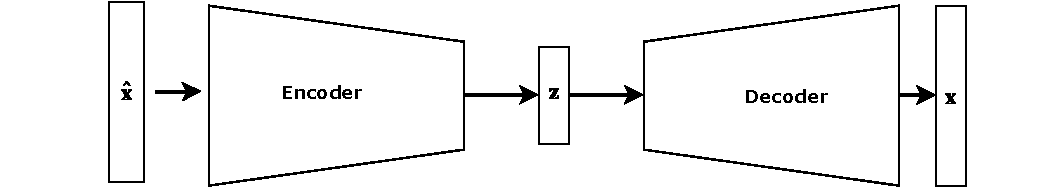
\includegraphics[width=\textwidth]{plots/autoencoder.pdf}
    \caption[Autoencoder schematic]{Schematic of an autoencoder model. A sample $\hat{\boldsymbol{x}}$ is compressed to a lower-dimensional representation $\boldsymbol{z}$, and is subsequently projected to the original space by the decoder to form a reconstruction. The tapered shape of trapezoid which represents the networks indicates if the network is compressing or uncompressing a representation.}
    \label{fig:autoencoder}
\end{figure}

\noindent An illustration of a general autoencoder architecture is included in figure \ref{fig:autoencoder}.

The objective is then to find the configuration of the two maps, $\phi$ and $\psi$, that gives the best possible reconstruction. That is the objective $\mathcal{O}$ for the model is given as

\begin{align}\label{eq:objective_autoenc}
  \mathcal{O} = \argmin_{\phi, \psi} \sum_i || \boldsymbol{x}_i - \phi(\psi( \boldsymbol{x}_i ))  ||^2
\end{align}

\noindent  As the name implies the encoder creates a lower-dimensional "encoded" representation of the input. A mean-squared-error cost optimizes this objective function in the event of real-valued data, but just as commonly through a binary cross-entropy for data normalized to the range $[0, 1]$. This representation can be useful for identifying whatever information-carrying variations are present in the data. An autoencoder can be thought of as an analogue to principal component analysis (PCA)\cite{Marsland2009}, which we introduced in chapter \ref{chap:fundament}. In practice, the non-linear maps, $\psi$ and $\phi$, are most often parametrized by neural networks. We refer to section \ref{sec:ANN} for a detailed discussion on deep learning and neural networks.

The autoencoder has previously been successfully implemented in de-noising tasks. More recently, the Machine Learning community discovered that one could impose a constraining term on the latent distribution to allow for the imposition of structure in the latent space. The goal in mind was to create a generative algorithm, a class of models used to sample from the distribution $P(\mathcal{X})$. For example, to generate bespoke images of houses. 

The first of these employed a Kullback-Leibler divergence to impose structure on the latent space. These models were dubbed variational autoencoders or VAEs by \citet{Kingma2013}. While VAEs lost the contest for preeminence as a generative algorithm to adversarial\footnote{Adversarial networks are a pair of networks where one aims to generate realistic samples, and the other aims to separate between fake and real samples} networks, they remain a fixture in the literature of expressive latent variable models with development focusing on the salience of the latent space \cite{Higgins2017}, \cite{Zhao}, \cite{Fertig}.

\section{The Variational Autoencoder}\label{sec:vae}

Initially presented by \citet{Kingma2013} the VAE is a twist upon the traditional autoencoder. Where the applications of an ordinary autoencoder largely extended to de-noising, with some authors using it for dimensionality reduction, the VAE seeks to control the latent space of the model. The goal of the VAE is then to be able to generate samples from the unknown distribution over the data. In this thesis, the generative properties of the algorithm are not of interest. Our efforts mainly concentrate on the latent space itself. Specifically, the focus is discerning whether class membership, be it a physical property or something more abstract\footnote{examples include discerning whether a particle is a proton or electron, or capturing the "five-ness" of a number in the handwritten digits MNIST dataset} is encoded in the space.

We begin this chapter with the discussion of the VAE as the framework for deriving the cost, and the methodology underpins the formalism on how we view the regularization of latent spaces.

\subsection{The variational autoencoder cost}

In section \ref{sec:intro_autoenc} we introduced the structure of the autoencoder. For the VAE, which is a more integral part of the technology used in the thesis, a more rigorous approach is warranted. We will here derive the loss function for the VAE in such a way that clarifies how we aim to impose a known structure of the latent space.

We begin by considering the family of problems encountered in variational inference, where the VAE takes its theoretical inspiration. Specifically, we will derive the VAE  as a solution to a Bayesian variational inference problem. Bayesian inference is a framework for linking some observed values $x$ to some hypothesized latent variable $z$. 

This family of techniques all begin with a consideration of the problem from Bayes' theorem. This theorem relates the probability of seeing our model given our data, $p(z|x)$ to the odds ratio of seeing our model $p(x|z)p(z)$ to the evidence $p(x)$. Bayes' rule is expressed mathematically as 

 \begin{equation}\label{eq:bayes}
 p(z| x) = \frac{p(x|z) p(z)}{p(x)}.
 \end{equation}

 \noindent The left-hand side is termed the posterior distribution. The posterior describes our updated knowledge given some prior belief (or hypothesis), $p(z)$ which expresses the probability of the model and the likelihood of seeing the data given the prior, $p(x|z)$. We recognize the likelihood from our introduction to information theory in \ref{sec:information}. The last part of this equation is the denominator which is commonly referred to as the evidence. It is also what causes the problem to be challenging. To see why we introduce some common re-writing tools used in statistical analysis. Beginning with the evidence, expressed as the integral of the joint distribution 

\begin{equation}
p(x, z) = p(x|z)p(z),
\end{equation}

\noindent such that

\begin{equation}\label{eq:evidence}
p(x) = \int_z p(x|z)p(z).
\end{equation}

\noindent The integral in the denominator of equation \ref{eq:bayes} is intractable for most interesting problems, as the space over $z$ is usually combinatorially large. 

Another standard tool for solving this problem is Markov chain Monte Carlo (MCMC) methods. In physics, this family of algorithms has been applied to solve many-body problems in quantum mechanics primarily by gradient descent on variational parameters \cite{Hjorth-Jensen}.

We can then summarize variational Bayesian methods as being techniques for estimating computationally intractable integrals as the one expressed in \ref{eq:evidence}. To derive an approximation to the evidence, we begin by introducing the KL-divergence. This function is a measure of how much two distributions are alike \cite{Kullback1951}. We define the KL-divergence from a probability measure P to another Q, by their probability density functions p, q over the set $x \in \mathcal{X}$ as

\begin{align}\label{eq:kl}
D_{KL} (P || Q) &= - \int^{\infty}_{-\infty} p(x) \log \left(\frac{p(x)}{q(x)}\right) dx, \\
&= \langle \log \left(\frac{p(x)}{q(x)} \right)\rangle_{p}.
\end{align}

\noindent In the context of the VAE, the KL-divergence is a measure of the quality of a model P approximating the true measure Q \cite{Burnham2002}. The first part of deriving the cost is then to introduce an approximation of the evidence. 

We introduce the evidence lower bound (ELBO) as an approximation to the evidence following the derivation laid out by \citet{Kingma2013}. The EBLO function is defined as 

\begin{equation}\label{eq:elbo}
ELBO(q) = \langle \log(p(z, x)) \rangle - \langle \log(q(z|x)) \rangle.
\end{equation}

\noindent To show that this function approximates the evidence we rewrite the ELBO in terms of the conditional distribution of $x$ given $z$

\begin{align}
ELBO(q) &= \langle \log(p(z)) \rangle +  \langle \log(p(x|z)) \rangle - \langle \log(q(z|x)) \rangle, \\
&=   \langle \log(p(x|z)) \rangle - D_{KL}(q(z|x) | p(z)).
\end{align}

\noindent Finally, the ELBO can be written as a lower bound on the evidence using Jensen's inequality (J) for concave functions. Mathematically we express the inequality as 

\begin{equation}
f(\langle x\rangle) \geq \langle f(x) \rangle.
\end{equation}

\noindent From the definition of the evidence we then have

\begin{align}
\log (p(x)) &= \log \int_z p(x|z) p(z), \\
&= log \int _z p(x|z) p(z) \frac{\psi(z|x)}{\psi(z|x)},\\
& = log \langle p(x|z) p(z)/ \psi (z|x) \rangle, \\
&  \stackrel{\mathclap{\text{(J)}}}{\geq} \langle \log (p(x|z) p(z)/ \psi(z|x))\rangle,\\
& = \langle \log(p(x|z))\rangle + \langle \log(p(z))\rangle  - \langle \log(\psi (z|x))\rangle, \\
\log (p (x)) &\geq \langle \log(p(x|z))\rangle - D_{KL}(\psi (z|x) || p(z)),
\end{align}

\noindent where we inserted $\psi$ to denote the encoder model. We have now shown that the ELBO is indeed a lower bound on the log evidence. 

 We can then move on to the VAE cost. We begin by defining $q(z|x)$ to be the posterior distribution over the latent variable $z \in \mathcal{Z}$, conditional on our data $x \in \mathcal{X}$ with evidence $p(x)$ and latent prior $q(z)$, with an associated probability measure $Q$ as per our notation above. Let then the parametrized distribution over the latent space enacted by the encoder be given as $\psi(z|x)$, and an associated probability measure $\Psi$. The quality of our encoder can then be decomposed as 

\begin{align}
D_{KL}(\Psi || Q ) &= \langle \log \left(\frac{\psi(z|x)}{q(z|x)}\right) \rangle_z, \\
&= \langle \log \left(\psi(z|x)- \log q(z|x)\right) \rangle_z.
\end{align}

\noindent From Bayes' rule, we can re-state the posterior by introducing the decoder $\phi(x|z)$. Continuing the derivation we then have 

\begin{align}
D_{KL}(\Psi || Q ) &=  \langle \log \left( \psi(z|x)\right)  - \log \left( \phi( x | z) q(z) \right) + \log (q(x))\rangle_z, 
\end{align}
\noindent where we identify that the evidence can be taken outside the expectation. Re-arranging the terms separates the model from the optimization targets 

\begin{align}
D_{KL}(\Psi || Q ) - \log q(x) &=  \langle \log \psi(z|x) - \log q(z) - \log \left( \phi( x | z)\right) \rangle_z, 
\end{align}

\noindent Note that the term $-\langle \log \left( \phi( x | z)\right) \rangle_z$ is the negative log-likelihood of our decoder network which we can optimize with the cross-entropy as discussed in section \ref{sec:LogReg}. We also identify that we can re-write the right side to include another KL divergence between the latent prior and the encoder. Flipping the sign then gives us the VAE cost

\begin{equation}\label{eq:vae_cost}
\log(p(x)) - D_{KL}(\Psi || Q )=  \langle \log \left( \phi( x | z)\right) \rangle_z - D_{KL}(\psi(z|x)|| q(z)).
\end{equation}
 
\noindent We are still bound by the intractable integral defining the evidence $q(x) = \int_z q(x, z)$ which is the same integral as in the denominator in equation \ref{eq:bayes}. We solve this problem by recognizing that the right-hand side is the ELBO and so we conclude that the VAE fits on the lower bound of the evidence.

\citet{Kingma2013} showed that this variational lower bound on the marginal likelihood of our data is feasibly approximated with a neural network when trained with backpropagation and gradient descent methods. That is, we estimate the derivative of the ELBO with respect to the neural network parameters, as described by the backpropagation algorithm in section \ref{sec:backpropagation} and iteratively improve the neural network with a gradient descent algorithm.

\section{Optimizing the variational autoencoder}\label{sec:vae_opt}

From equation \ref{eq:vae_cost}, we observe that the optimization is split in two. The first is a reconstruction term that approximates the log evidence, which we can train with a squared error or cross-entropy cost. Secondly, we have a divergence term over the parametrized and theoretical latent distribution. We want to simplify the second to conserve computational resources. Thankfully this is computationally cheap given a specific prior latent distribution. Let the target distribution $p(z | x) $ be a multivariate normal distribution with zero means and a diagonal unit variance matrix, i.e. $p(z | x) \sim  \mathcal{N}(\boldsymbol{0}, \boldsymbol{I})$. And accordingly the neural network approximation then follows $\psi(z | x) \sim \mathcal{N}(\mu, \Sigma)$. The normalized probability density function for the normal Gaussian is defined as 

\begin{equation}
p(\boldsymbol{x}) = \frac{1}{(2\pi)^{n/2}|\Sigma|^{1/2}}exp(-\frac{1}{2}(\boldsymbol{x} - \mathbb{\mu})^T\Sigma^{-1}(\boldsymbol{x}-\mu)),
\end{equation}

\noindent and the Kullback-Leibler divergence for two multivariate Gaussians is given by 


\begin{equation}
\hspace*{-0.1in}
D_{KL}(p_1|| p_2 ) = \frac{1}{2} \left( \log \frac{|\Sigma_2|}{|\Sigma_1|} -n + tr(\Sigma^{-1}_2 \Sigma_1) + (\mu_2 - \mu_1)^T\Sigma_2^{-1}(\mu_2 - \mu_1) \right),
\end{equation}

\noindent which we derive in appendix \ref{appendix:kl_gauss}. Substituting $p_1$ and $p_2$ with the model distribution $\psi(z|x)$ and a latent prior $p(\boldsymbol{z}) \sim \mathcal{N}(\boldsymbol{0}, \boldsymbol{I})$ we get 

\begin{align*}
D_{KL}(q||p) &= \frac{1}{2} \left( - \log {|\Sigma_1|} -n + tr(I \Sigma_1) + \mu_2 ^TI\mu_2 \right) \\
&= \frac{1}{2} \left( - \log {|\Sigma_1|} -n + tr(\Sigma_1) + \mu_2 ^T\mu_2 \right),
\end{align*}

\noindent or more conveniently

\begin{equation}\label{eq:kl_opt}
D_{KL}(q||p) = \frac{1}{2} \sum_i -\log \sigma_i^2 - 1 + \sigma^2_i + \mu_i^2 .
\end{equation}

\noindent We note that equation \ref{eq:kl_opt} satisfies the equality that the divergence is zero when the target and model distributions are equal. The VAE model can then be enacted with a pair of neural networks acting as an encoder and decoder. To parametrize the sample, we compute a mean vector $\mu$ and a variance vector $\sigma^2$ from the encoded representation. The latent sample is then given as 

\begin{equation}
\boldsymbol{z} = \boldsymbol{\mu} + \boldsymbol{\sigma}^2 \cdot \epsilon,
\end{equation} 

\noindent where $\epsilon$ is a stochastic vector drawn from $\mathcal{N}(\boldsymbol{0}, \boldsymbol{1})$. A schematic of a VAE model is shown in figure \ref{fig:var_autoencoder}.

An essential feature of the Kullback-Leibler divergence is that it operates point-wise on the probability densities. This aspect was the point of contention in the paper by \citet{Zhao}. In the paper, the authors propose alternate measures for regularizing the latent space. They argue that the KL-divergence is problematic where the probability of the target distribution is close to zero. As a remedy, the authors propose to compare the moments of the distribution and minimize their difference. 


\begin{figure}[tb]
    \centering
    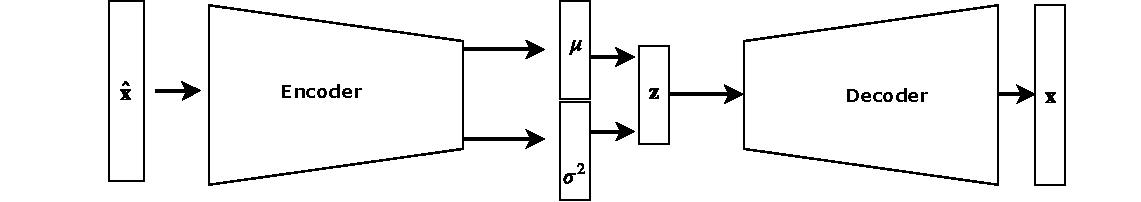
\includegraphics[width=\textwidth]{plots/variational_autoenc.pdf}
    \caption[Variational autoencoder schematic]{Schematic of a variational autoencoder model. A sample $\hat{\boldsymbol{x}}$ is compressed to a lower-dimensional representation $\boldsymbol{z}$, which is parametrized by a mean vector, $\boldsymbol{\mu}$, and a variance vector $\boldsymbol{\sigma}^2$. Subsequently, we reconstruct the original input with the decoder.}
    \label{fig:var_autoencoder}
\end{figure}


\subsection{Mode collapse}\label{sec:mode_collapse}

When training a VAE, we are balancing the evidence and prior latent distribution loss terms. \citet{Kingma2013} note that equation \ref{eq:vae_cost} is unbalanced in favor of the latent space regularization. As a consequence, the un-weighted loss suffers from mode collapse. When the reconstruction is under-valued in the optimization, the model will quickly learn the prior, without encoding the input. As the prior has become uninformative, the decoder proceeds to learn a rough representation. This representation usually covers as many of the outputs as possible. Mode collapse can then often be visually identified by the output being a vague cloud that looks like an average of all the data. 
